\section{Supplimentary Experiments on Reinforcement Learning}

\subsection{Additional Ablation Study on Advantage Estimation}

Here are some other supplimentary experiments on RL absent in the main body. They provide more evidence on the theoretical results obtained by our analysis and beyond.

\begin{figure}[htb]
  \centering
  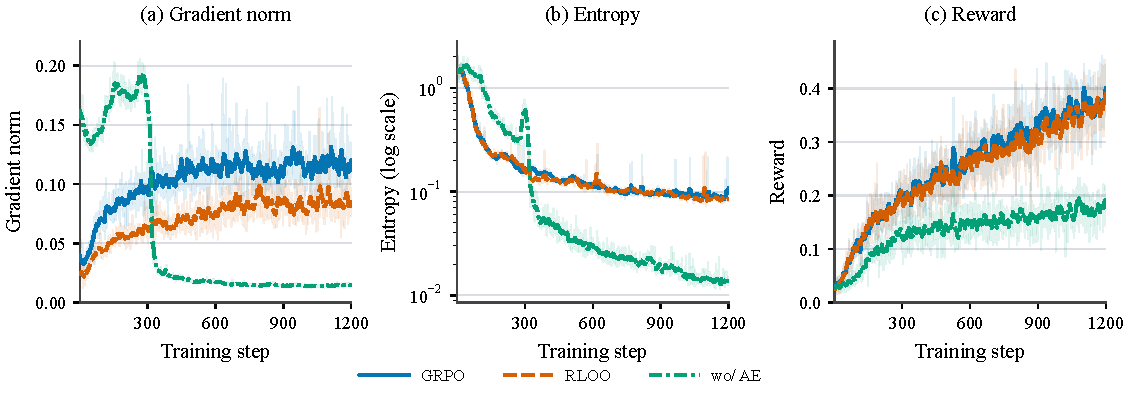
\includegraphics[width=\linewidth]{media/adv_estimators_comparison_smollm.pdf}
  \caption{The ablation study on the advantage estimation on SmolLM2-360M-Instruct~\citep{allal_smollm2_2025} and GSM8K~\citep{cobbe_training_2021} dataset. with batchsize 128, n\-samples 4 and AdamW optimizer with learning rate 1e-5.}
  \label{fig:supp-exp-rl-smollm}
\end{figure}

In Figure~\ref{fig:supp-exp-rl-smollm} we also examined the variance effect on smaller models like SmolLM2-360M-Instruct. We used similar training settings like that in \citet{tajwar_maximum_2026}. We can see that advantage estimation methods effectively prevents entropy collapse and stabilizes the training process. These experiments share the following hyperparameter settings in AReaL~\citep{fu_areal_2025}, unmentioned hyperparameters are kept the same as the default setting:

\begin{itemize}
  \item seed: 1
  \item batchsize: 128
  \item n\_samples: 4
  \item total\_train\_steps: 1200
  \item actor.optimizer.lr: 1e-5
  \item actor.reward\_scaling: 2.0
  \item actor.reward\_bias: -0.5
\end{itemize}

\subsection{Additional Results on Conditional KL Restriction}

\begin{figure}[htb]
  \centering
  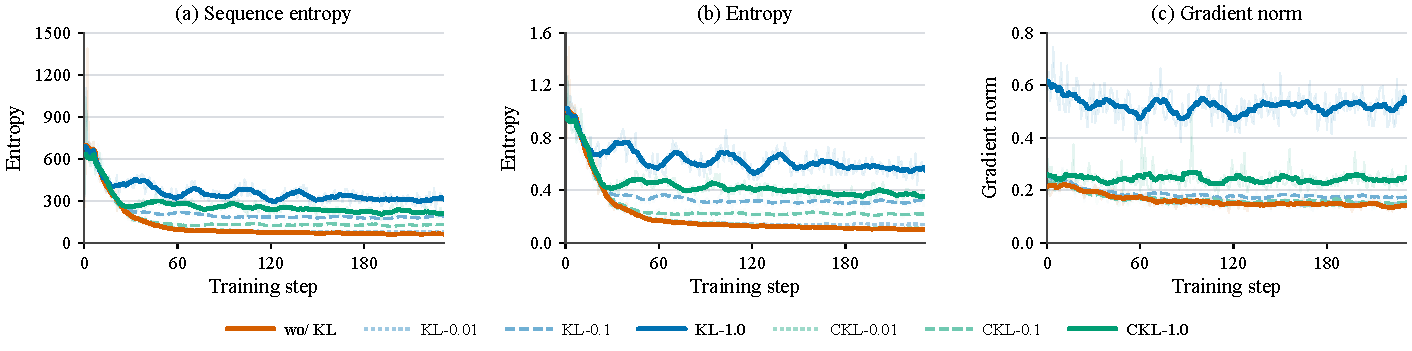
\includegraphics[width=\linewidth]{media/conditional_kl_metrics.pdf}
  \caption{Additional metrics on the comparison of KL and CKL restrictions.}
  \label{fig:addi-kl-ckl}
\end{figure}

The results in Figure~\ref{fig:addi-kl-ckl} come from the same set of experiments as that in Figure~\ref{fig:kl-ckl-comparison}. We can see that the sequence-level entropy showed the same decreasing trend as that of token-level entropy. Recall the entropy decomposition in Lemma~\ref{lem:rl-target-entropy}, the entropy of a model in RL is only comparable if they have similar accuracy. Otherwise the entropy value may not directly reflect the collapse in diversity. The gradient norm behavior of these experiments also provides some explanation on the advantage of CKL restriction. With high restriction strength, the gradient of CKL is much more modest while it still preserves the diversity very well.

These experiments adopts these hyperparameter settings, while unmentioned ones use the default value in AReaL~\citep{fu_areal_2025}:

\begin{itemize}
  \item seed: 1
  \item batchsize: 128
  \item n\_samples: 4
  \item total\_train\_epochs: 4
  \item actor.optimizer.lr: 1e-6
  \item actor.reward\_scaling: 2.0
  \item actor.reward\_bias: -0.5
  \item actor.kl\_estimator: "k1"
\end{itemize}


\begin{figure}[htb]
  \centering
  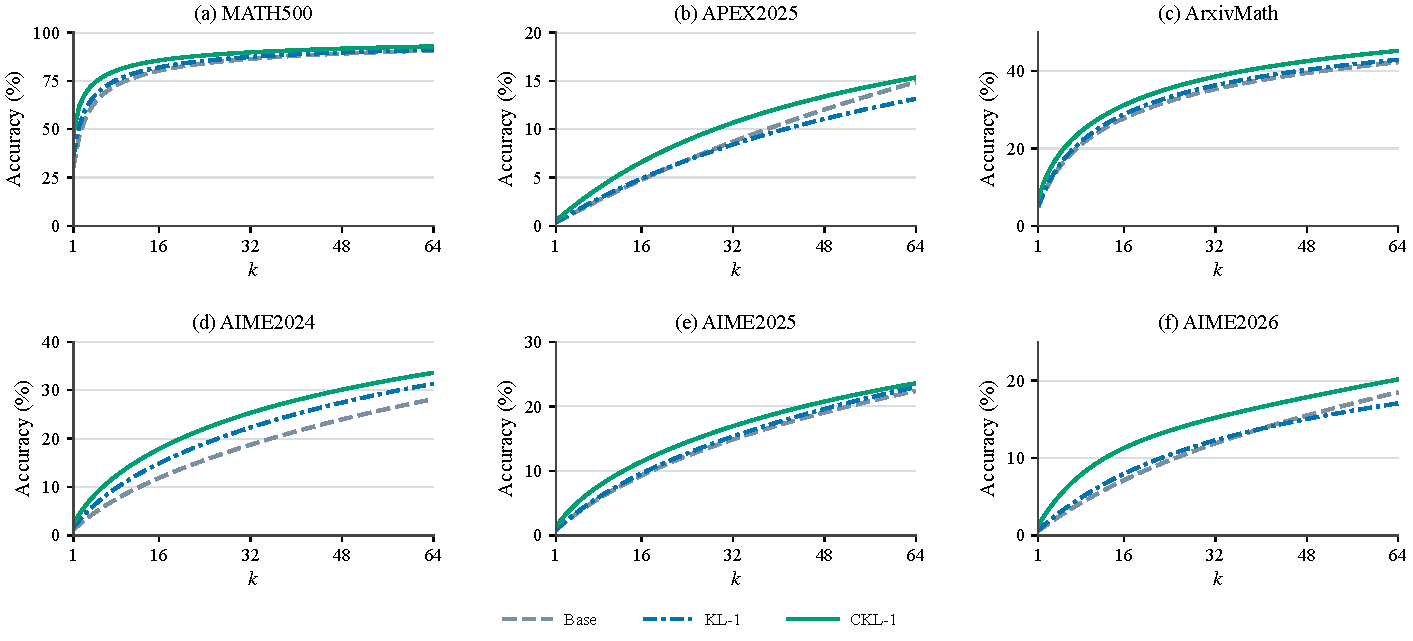
\includegraphics[width=\linewidth]{media/passk_comparison_appendix.pdf}
  \caption{Extended pass@k performance of models trained with KL or CKL regularization. CKL regularization also preserves more learning potential in the sense of pass@k performance compared with KL regularization with the same strength. The evaluation settings is the same as that used in AReaL training pipeline.}
  \label{fig:passk-eval-full}
\end{figure}
